\section{Model of L\'evy Walks/Flights in cognition, incorporating memory}


\begin{figure}[h!]
\begin{center}
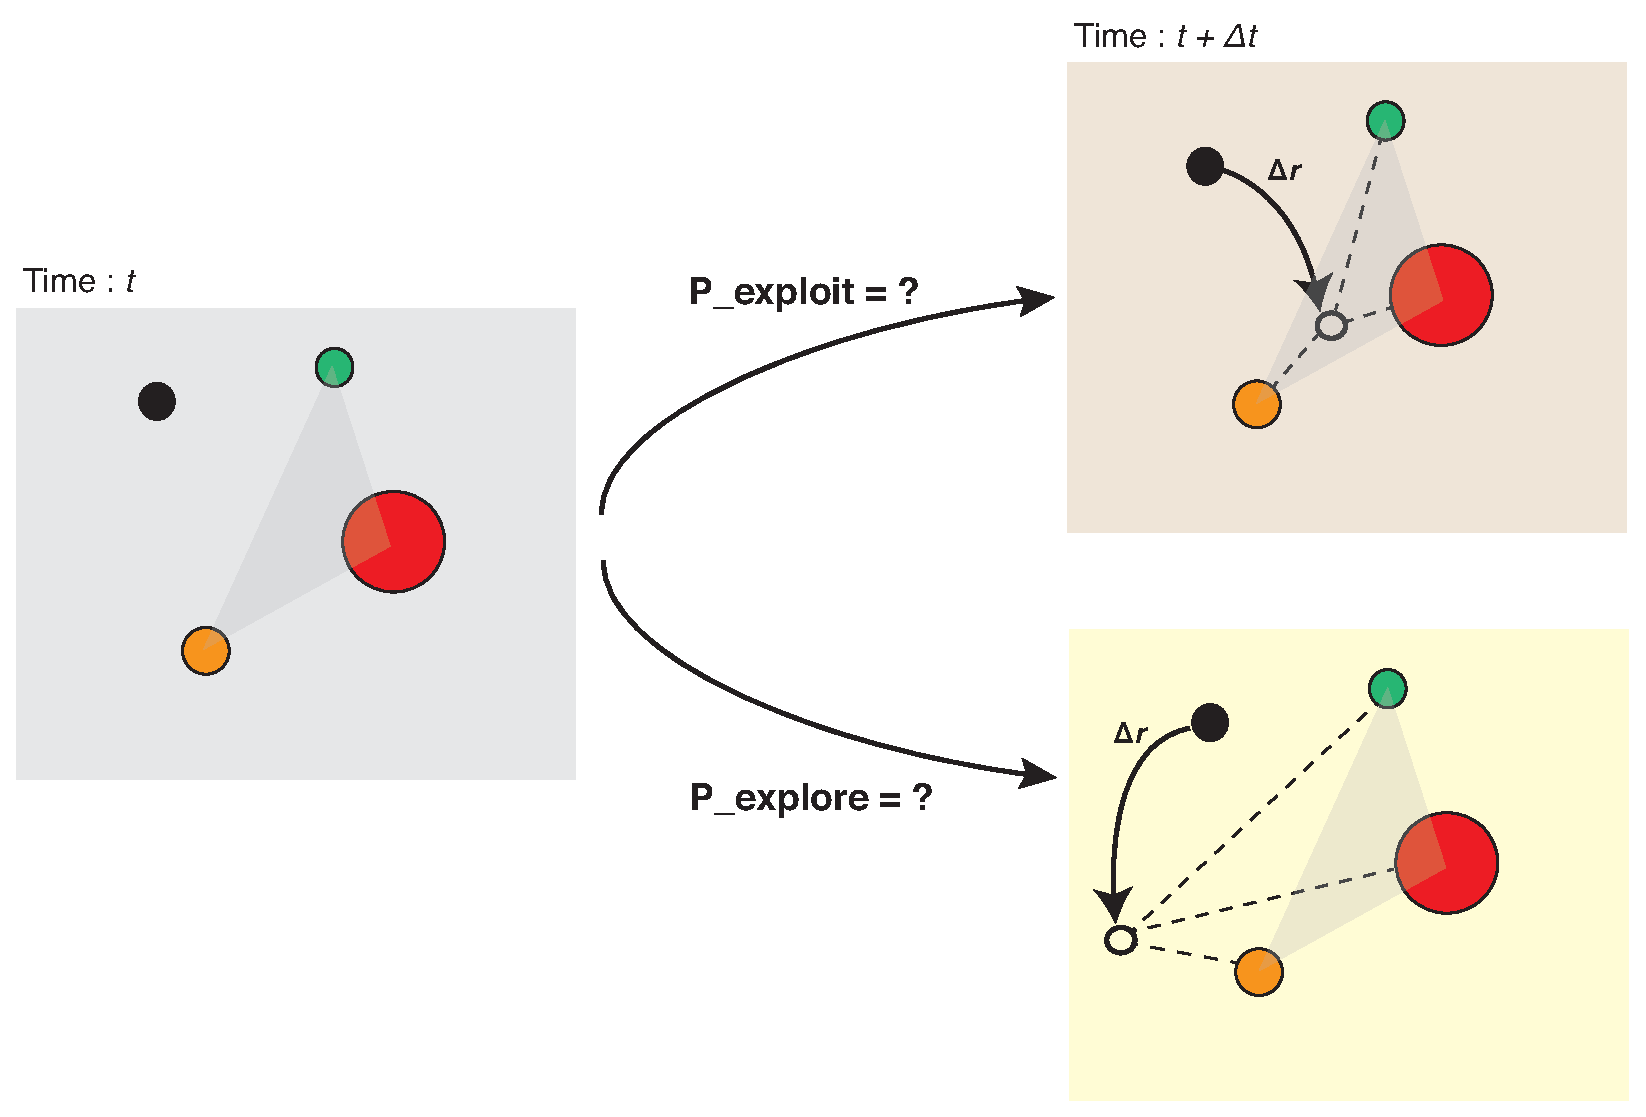
\includegraphics[width=10cm]{figures/schematic_displacement.eps}
\caption{\footnotesize{2-dimensional schematic description of the {\it L\'evy flying mind} model ({\bf ``Proportional Attraction"}): At each time step, the individual must choose between remaining in the solution envelope that has already been explored and exploring outside the currently known solution envelope.  We assign some probability $p$ (a number between 0 and 1) to the participant's decision of staying in the explored envelop and probability $1-p$ to the decision to explore outside that envelop.  If it is harder to find solutions that offer a balanced re-combination of previous solutions than to think out-of-the-box and propose solutions outside of the current solution envelope, then $p < \frac{1}{2}$ else $p \geq \frac{1}{2}$.}}
\label{fig:schematic}
\end{center}
\end{figure}

%\section{What can we learn from stylised facts regarding timing ?}

%\section{Discrete cascading models and recombination of knowledge}



